\subsection{The Turing machine $M_\text{paren}$}

This Turing machine should recognize sequences of balanced parentheses. 

\subsubsection{Description}

\paragraph{High-level description}
Repeatedly, we move right to the next $)$, replace it with $X$, then we move left until we find the next $($ and replace it with $X$. 

If when we are looking for a $)$ and we reach the end of the tape ($\_$), we accept if the tape only contains $X$. Note that we need to introduce a special start of tape symbol and take care of the ramifications of introducing this new symbol.

\paragraph{Implementation-level description}
$M_{\text{paren}}=$
``on input $w \in \{(,)\}^*$:

\begin{enumerate}
    \item If the initial cell is blank, accept; if it is $)$, reject. Otherwise, replace the $($ with $Y$.
    \item Sweep right until the next $)$ and replace it with $X$. 
        \begin{itemize}
            \item If in sweeping right we encounter $\_$, scan the tape left until $\$$ and reject if we encounter any $($, $)$ or $Y$. If, however, we do reach $\$$, accept.
        \end{itemize}
    \item Sweep left until the next $($ and replace it with $X$. Or, if we reach $Y$, replace it with $\$$. In either case, repeat from step 2.
        \begin{itemize}
            \item If in sweeping left we encounter $\$$, reject.''
        \end{itemize}
\end{enumerate}

Notice that the tape alphabet $\Gamma=\{(,),X,Y,\$\}$; it introduces three new letters.

\subsubsection{Theoretical analysis of complexity}

For all $n\geq 0$, there exists a particular input word $x \in \{(,)\}^n$ that maximizes the number of steps that $M_\text{paren}$ must perform until it halts, i.e. all other input words of that length either need the same number of steps or fewer. 

This worst-case scenario arises when $M_\text{paren}$ must:

\begin{itemize}
    \item sweep the longest distances because this causes more transitions; and
    \item perform the most sweeps because the input word cannot be rejected (or must be rejected as late as possible.
\end{itemize}

We find that the worst possible input word is a sequence of strictly nested parentheses because this input word satisfies both conditions.
Formally, these words are
$x_n = \textbf{(}^{\lceil n/2 \rceil} \textbf{)}^{\lfloor n/2 \rfloor}$,
i.e. open parentheses followed by the same number of close parentheses, prepended by an additional open parenthesis if the length of $x$ should be odd. 

We will now attempt to define the function $f(n)$ that returns the maximum number of transitions made by the TM for any word of length $n$.

\begin{wrapfigure}{r}{0.25\textwidth}
    \centering
    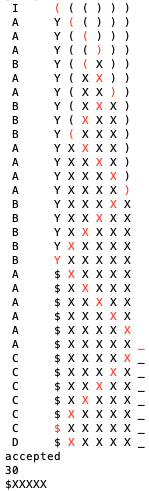
\includegraphics[width=2.5cm]{images/screenshots/paren.png}
    \vspace{-2cm}
\end{wrapfigure}

\paragraph{Complexity for even length words}

For even $n$:

\begin{itemize}
    \item we reach the first $)$ after moving right to the middle of the word ($n/2$ steps);
    \item we then move left $i_1=1$ time, right $i_2=2$ times, left $i_3=3$ times, ..., until we move right $i_n=n$ times (totalling $\sum_{i=1}^{n}{i}$ steps);
    \item at that point we reach $\_$, so we need to move left to the beginning of the word to verify that we have crossed of all parenthesis ($n$ steps);
    \item arriving at the left end of the tape ($\$$), we accept the word. 
\end{itemize}

Counting the steps, we obtain
$$ f_{\text{even}}(n) = \frac{n}{2} + \sum_{i=1}^{n}{i} + n.$$

Using the formula for sums of arithmetic sequences, we simplify to
\begin{align*} 
    f_{\text{even}}(n)
    &= \frac{n}{2} + \frac{n}{2} \left( 1+n \right) + n \\
    &= \frac{n^2}{2} + 2n.
\end{align*}


This can be visually verified by running \code{./runtm -v} on the \code{paren.tm} machine with an apprpriate input word. 
The \code{-v} option will print the tape at each state along with the position of the read head marked in red. 
The screenshot on the right shows the operation on the input \code{((()))}.


\paragraph{Complexity for odd length words}
For input words of the form $x_n=(^{\lceil n/2 \rceil} )^{\lfloor n/2 \rfloor}$:
\begin{itemize}
    \item we find the first $)$ after $(n+1)/2$ steps;
    \item then we follow the same procedure (move left and right from $i_1=1$ to $i_n=n-1$) (totalling $\sum_{i=1}^{n-1}{i}$ steps);
    \item at that point we reach $\_$ and need to move left to the beginning of the word ($n$ steps), concluding that that the word should be rejected.
\end{itemize}

We obtain
\begin{align*} 
    f_{\text{odd}}(n)
    &= \frac{n+1}{2} + \sum_{i=1}^{n-1}{i} + n\\
    &= \frac{n+1}{2} + \frac{n-1}{2} \left( 1+n-1 \right) + n \\
    &= \frac{n^2}{2} + n + \frac{1}{2}.
\end{align*}


\paragraph{Complexity class}
For all integers $n>1$, $f_{\text{even}}(n) > f_{\text{odd}}(n)$ because
$$
\frac{n^2}{2} + 2n
>
\frac{n^2}{2} + n + \frac{1}{2}.
$$

That only leaves us to consider $n=0$, but in this case $f_{\text{even}}$ applies, so for practical purposes $f_\text{even}(n)>f_\text{odd}(n) \ \forall n$, so we can conclude that $M_\text{paren}$ is in the complexity class
$$
    \text{DTIME}\left( \frac{n^2}{2} + 2n \right).
$$

Therefore the TM has $\mathcal{O}(n^2)$ complexity.

\subsubsection{Practical analysis of complexity}

The theoretical results are evident in practical trials. The data collected in \code{data/paren-nested.csv} confirms the findings of $f_\text{odd}$ and $f_\text{even}$ (the values were cross-checked). Furthermore, the plot below shows how this worst-case scenario behaves as a plot of $n$ against the number of transitions made by the machine. 

\begin{center}
    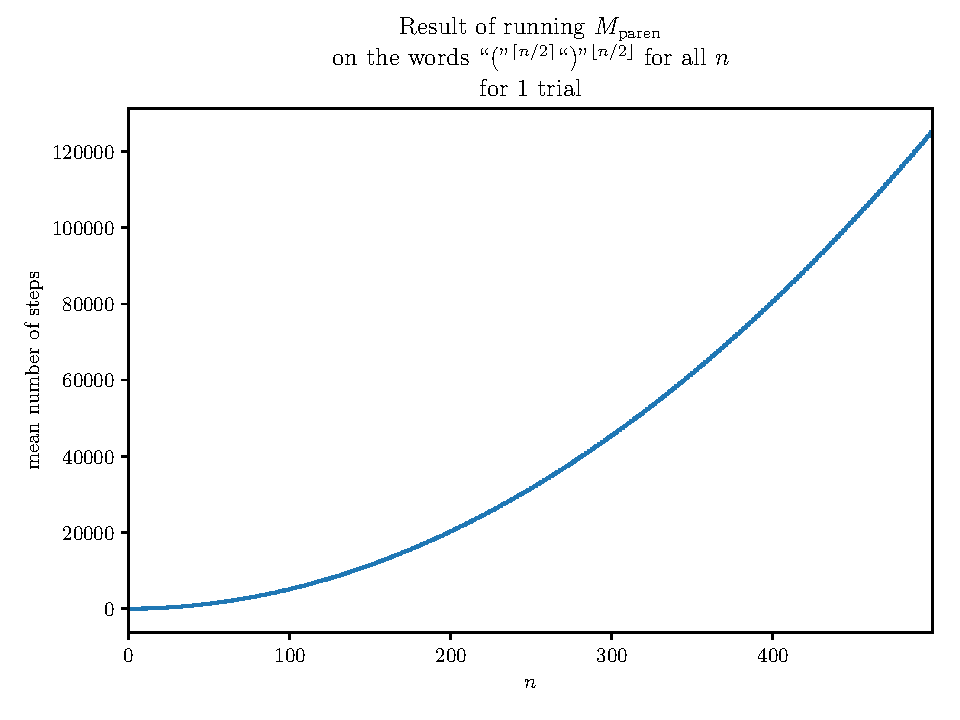
\includegraphics[width=\textwidth]{plots/paren-nested.pdf}
\end{center}

Other types of input words were also tested; please refer to the plots in section \ref{plots_paren}, as well as the CSV data in \code{data/paren-*.csv}. 